\section{Introduction}
I have spent the majority of my time this week deploying, testing DLib\cite{dlib} and YOLO framework.

\section{DLib}
\subsection{Installation}
To effectively manage different environments on my computer, I used Miniconda to install new frameworks. Here is the \href{https://raw.githubusercontent.com/tlvu2697/miniconda-scripts/master/dlib-setupenv.sh}{script} to install DLib environment via Miniconda.

Installation:
	\begin{lstlisting}
    curl https://raw.githubusercontent.com/tlvu2697/
miniconda-scripts/master/dlib-setupenv.sh | bash
	\end{lstlisting}

\subsection{Face Detector}
DLib provided a python example of Face Detector \href{http://dlib.net/face_detector.py.html}{here} for everybody to follow up. I referred to the example above and also made some changes to add bounding box to outputs.

DLib's Face Detector algorithm provided 2 thresholds to adjust by myself. The first threshold was the Upsampling threshold, which indicated how many times we wanted to upsample the image, that would make the input image bigger and allow us to detect more faces. The second threshold was the Detection threshold, where a negative value would return more detections and a positive value fewer.

Here were some results that I got by using DLib's Face Detector algorithm, with several Upsampling thresholds from 1 to 5, and two Detection thresholds which were the default threshold provided by DLib and my one of -1.

\newpage
\begin{SCfigure}[0.5][!ht]
\caption{One person with straight face}
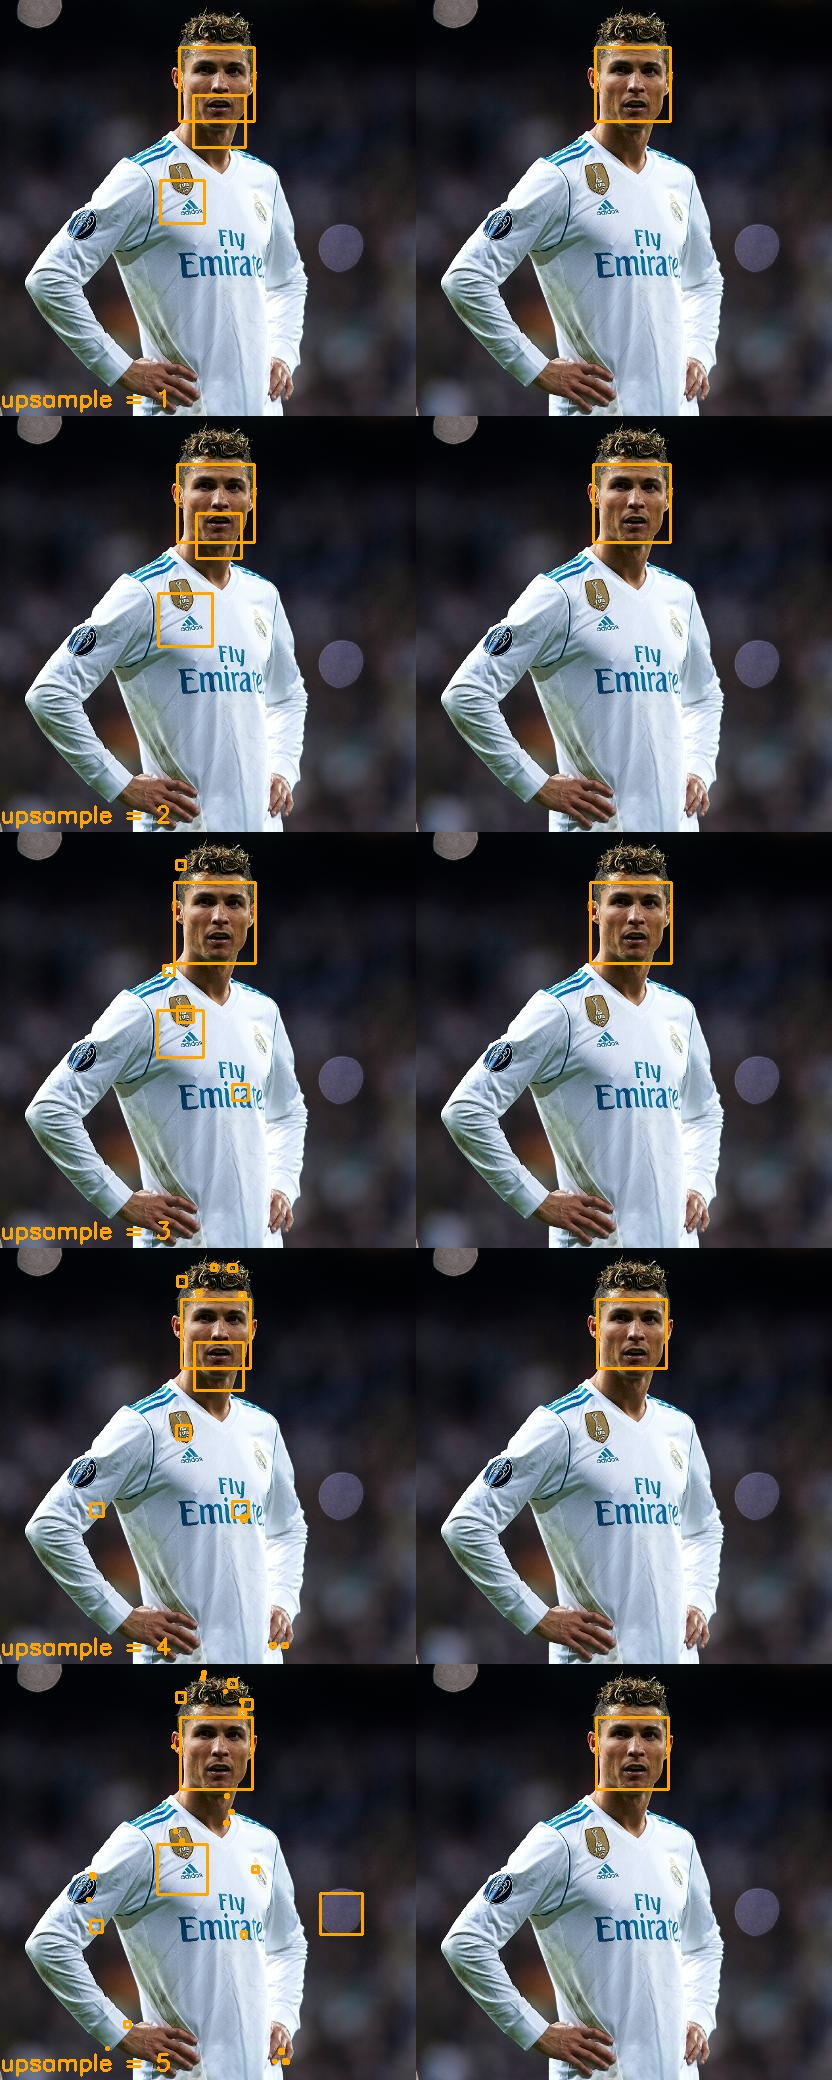
\includegraphics[height=0.9\textheight,keepaspectratio]{week3-dlib-face-detector-1.jpg}
\end{SCfigure}
In this case, algorithm worked well regardless of any Upsampling thresholds.

\newpage
\begin{SCfigure}[0.5][!ht]
\caption{One person with side face}
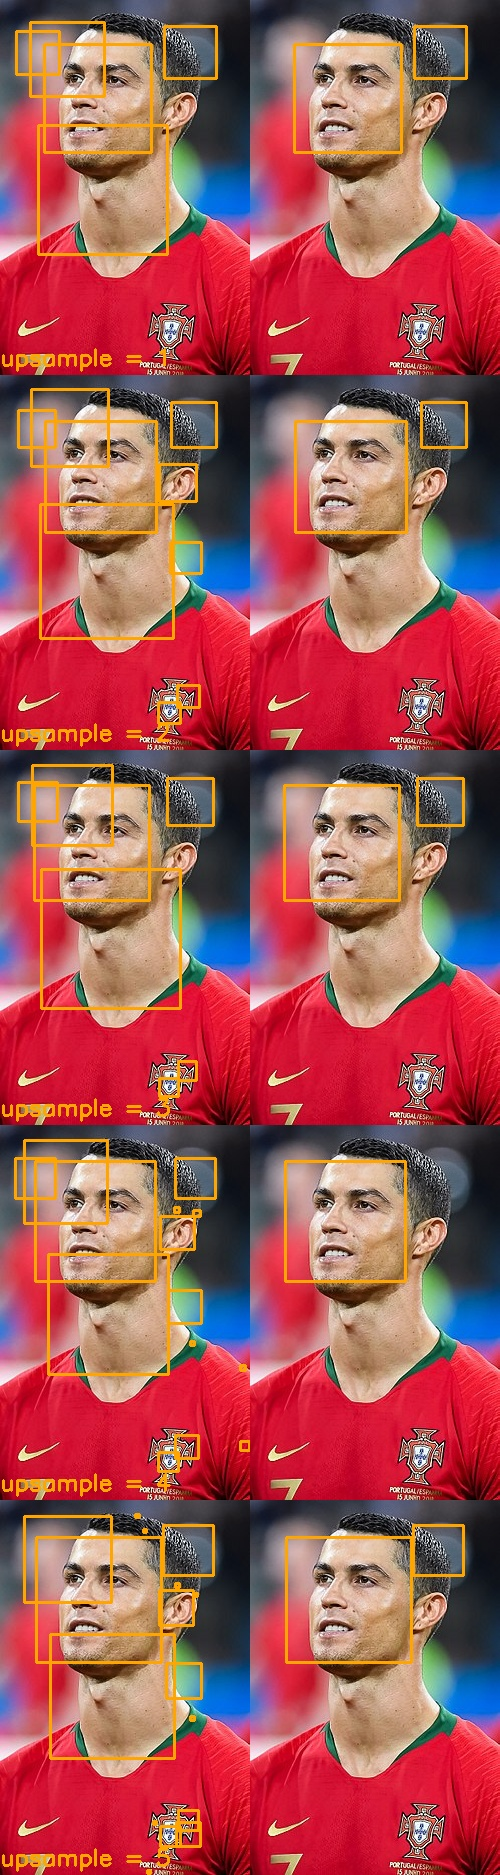
\includegraphics[height=0.9\textheight,keepaspectratio]{week3-dlib-face-detector-2.jpg}
\end{SCfigure}
In this case, the only Upsampling threshold that worked well was 4 while the others also successfully detected the right face, but there was one redundant detection.

\newpage
\begin{figure}[!ht]
\centering
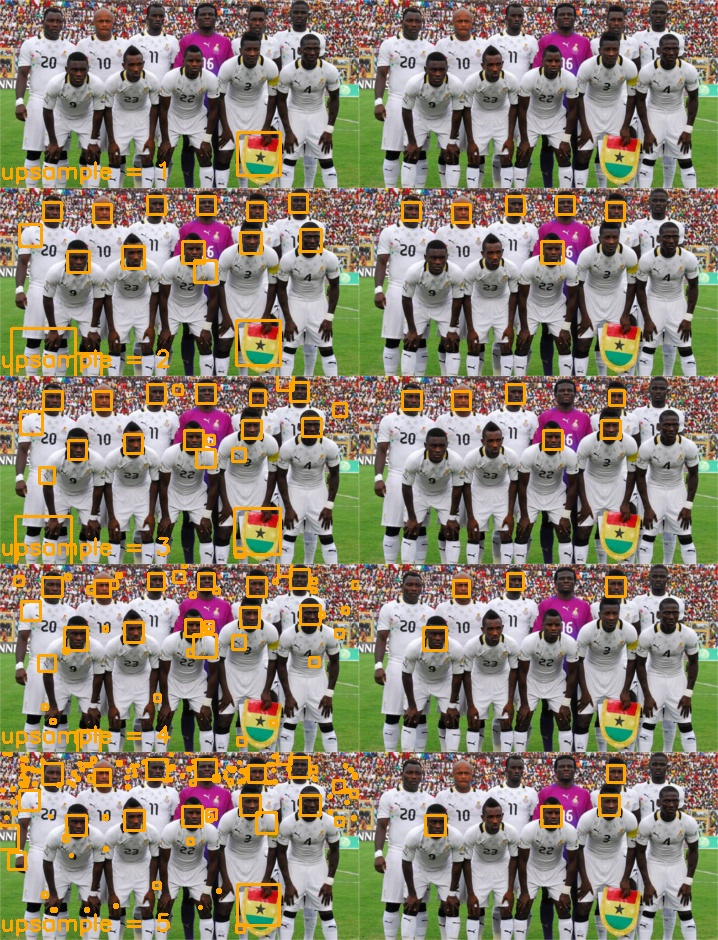
\includegraphics[width=\textwidth]{week3-dlib-face-detector-3.jpg}
\caption{Multi people with resolution of 359x188}
\end{figure}
In this case, the default Upsampling threshold which was 1 completely failed to detect faces. When Upsampling threshold increased, DLib was being able to detect more faces, but the result was still not so good. We could see that DLib successfully detected potential faces, but after filtering the result was not so good as expect.

\newpage
\begin{figure}[!ht]
\centering
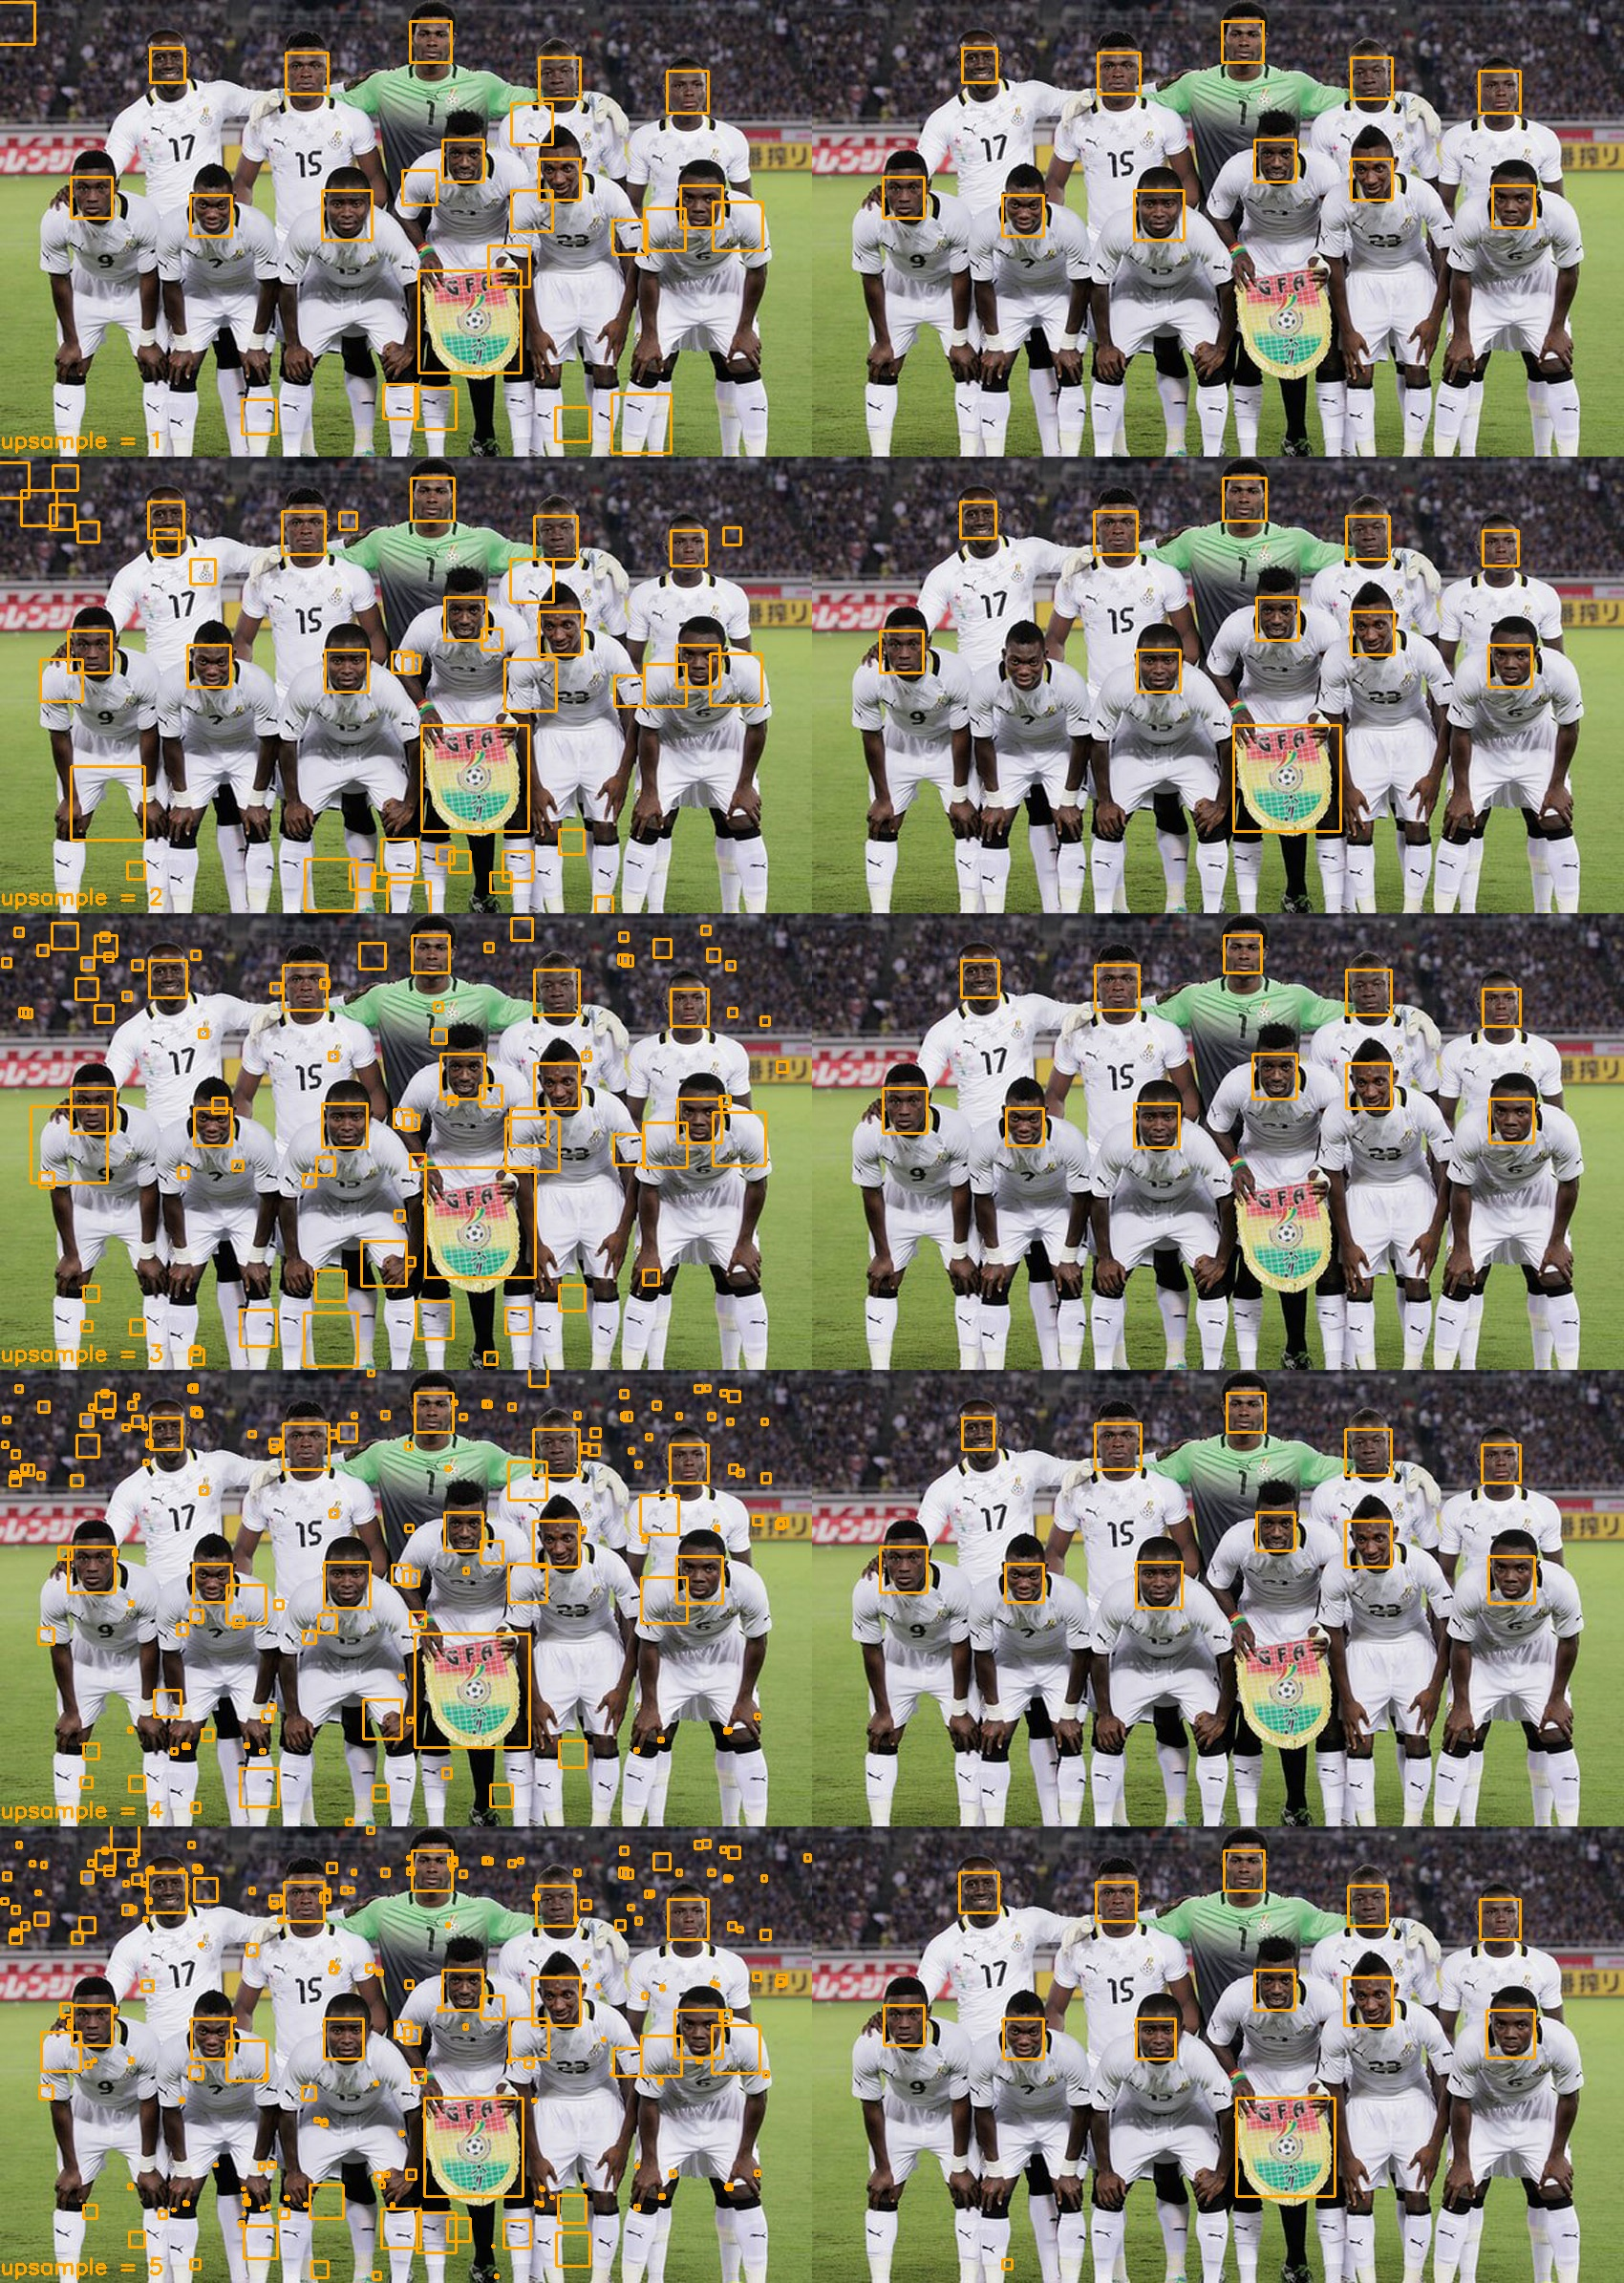
\includegraphics[width=\textwidth]{week3-dlib-face-detector-4.jpg}
\caption{Multi people with resolution of 850x478}
\end{figure}
In this case, the default Upsampling threshold which was 1 already worked so good. But when Upsampling threshold increased, there were some cases that DLib wrongly detected the flag as a face.

\newpage
\subsection{Face Recognition}
DLib provides a python example of Face Recognition \href{http://dlib.net/face_recognition.py.html}{here} to follow. For this algorithm I just focused on how to run it.

DLib also provides trained facial shape predictor and trained recognition model which can be download at:
\begin{itemize}
\item Shape predictor: \href{http://dlib.net/files/shape_predictor_5_face_landmarks.dat.bz2}{here}
\item Face recognition model: \href{http://dlib.net/files/dlib_face_recognition_resnet_model_v1.dat.bz2}{here}
\end{itemize}

The mission of this algorithm is to take input as an image and make output of a distinct 128 elements vector for each input person.

How to run:
\begin{lstlisting}
    python face_recognition.py shape_predictor.dat 
dlib_face_recognition_resnet_model_v1.dat image_dir/
\end{lstlisting}

\begin{figure}[!ht]
\centering
\begin{subfigure}{0.3\textwidth}
  \centering
  
\includegraphics[height=0.2\textheight,keepaspectratio]{week3-input-dlib-face-recognition-1.jpg}
  \caption{Input}
\end{subfigure}%
\begin{subfigure}{0.7\textwidth}
  \centering
  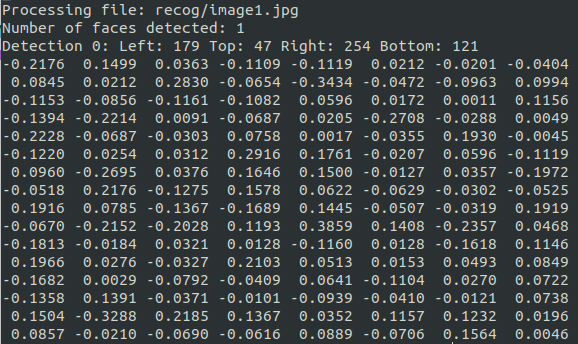
\includegraphics[height=0.2\textheight,keepaspectratio]{week3-dlib-face-recognition-1.png}
  \caption{Output}
\end{subfigure}
\caption{Face recognition example}
\end{figure}

\subsection{Problems}
I could not find out any guide to build DLib with GPU support. So I don't know whether DLib supports GPU or not.

I don't know what to do next with the 128 elements vector provided by Face Recognition algorithm, I guess that I can use a k-d tree (k == 128) to make a recognition system.

How can we evaluate the Face Detection and Face Recognition performance? And how to test their correctness?


\newpage
\section{YOLO}
\subsection{Installation}
YOLO can be built with CUDA to run on GPU which is much faster than CPU. You must have CUDA installed on your machine to build YOLO with CUDA option.

I already wrote a script to make the CUDA installation process easier. Follow the GPU installation below for more details.

Installation (CPU):
\begin{lstlisting}
    git clone https://github.com/pjreddie/darknet
    cd darknet
    make
\end{lstlisting}

Installation (GPU):
\begin{lstlisting}
    # Install CUDA first
    curl https://raw.githubusercontent.com/tlvu2697/colab-
scripts/master/cuda80-setup.sh | bash

    git clone https://github.com/pjreddie/darknet
    cd darknet

    # Change the first line of the Makefile to GPU=1
    make
\end{lstlisting}

\newpage
\subsection{Object Detection}
\begin{figure}[!ht]
\centering
\begin{subfigure}{1\textwidth}
  \centering
  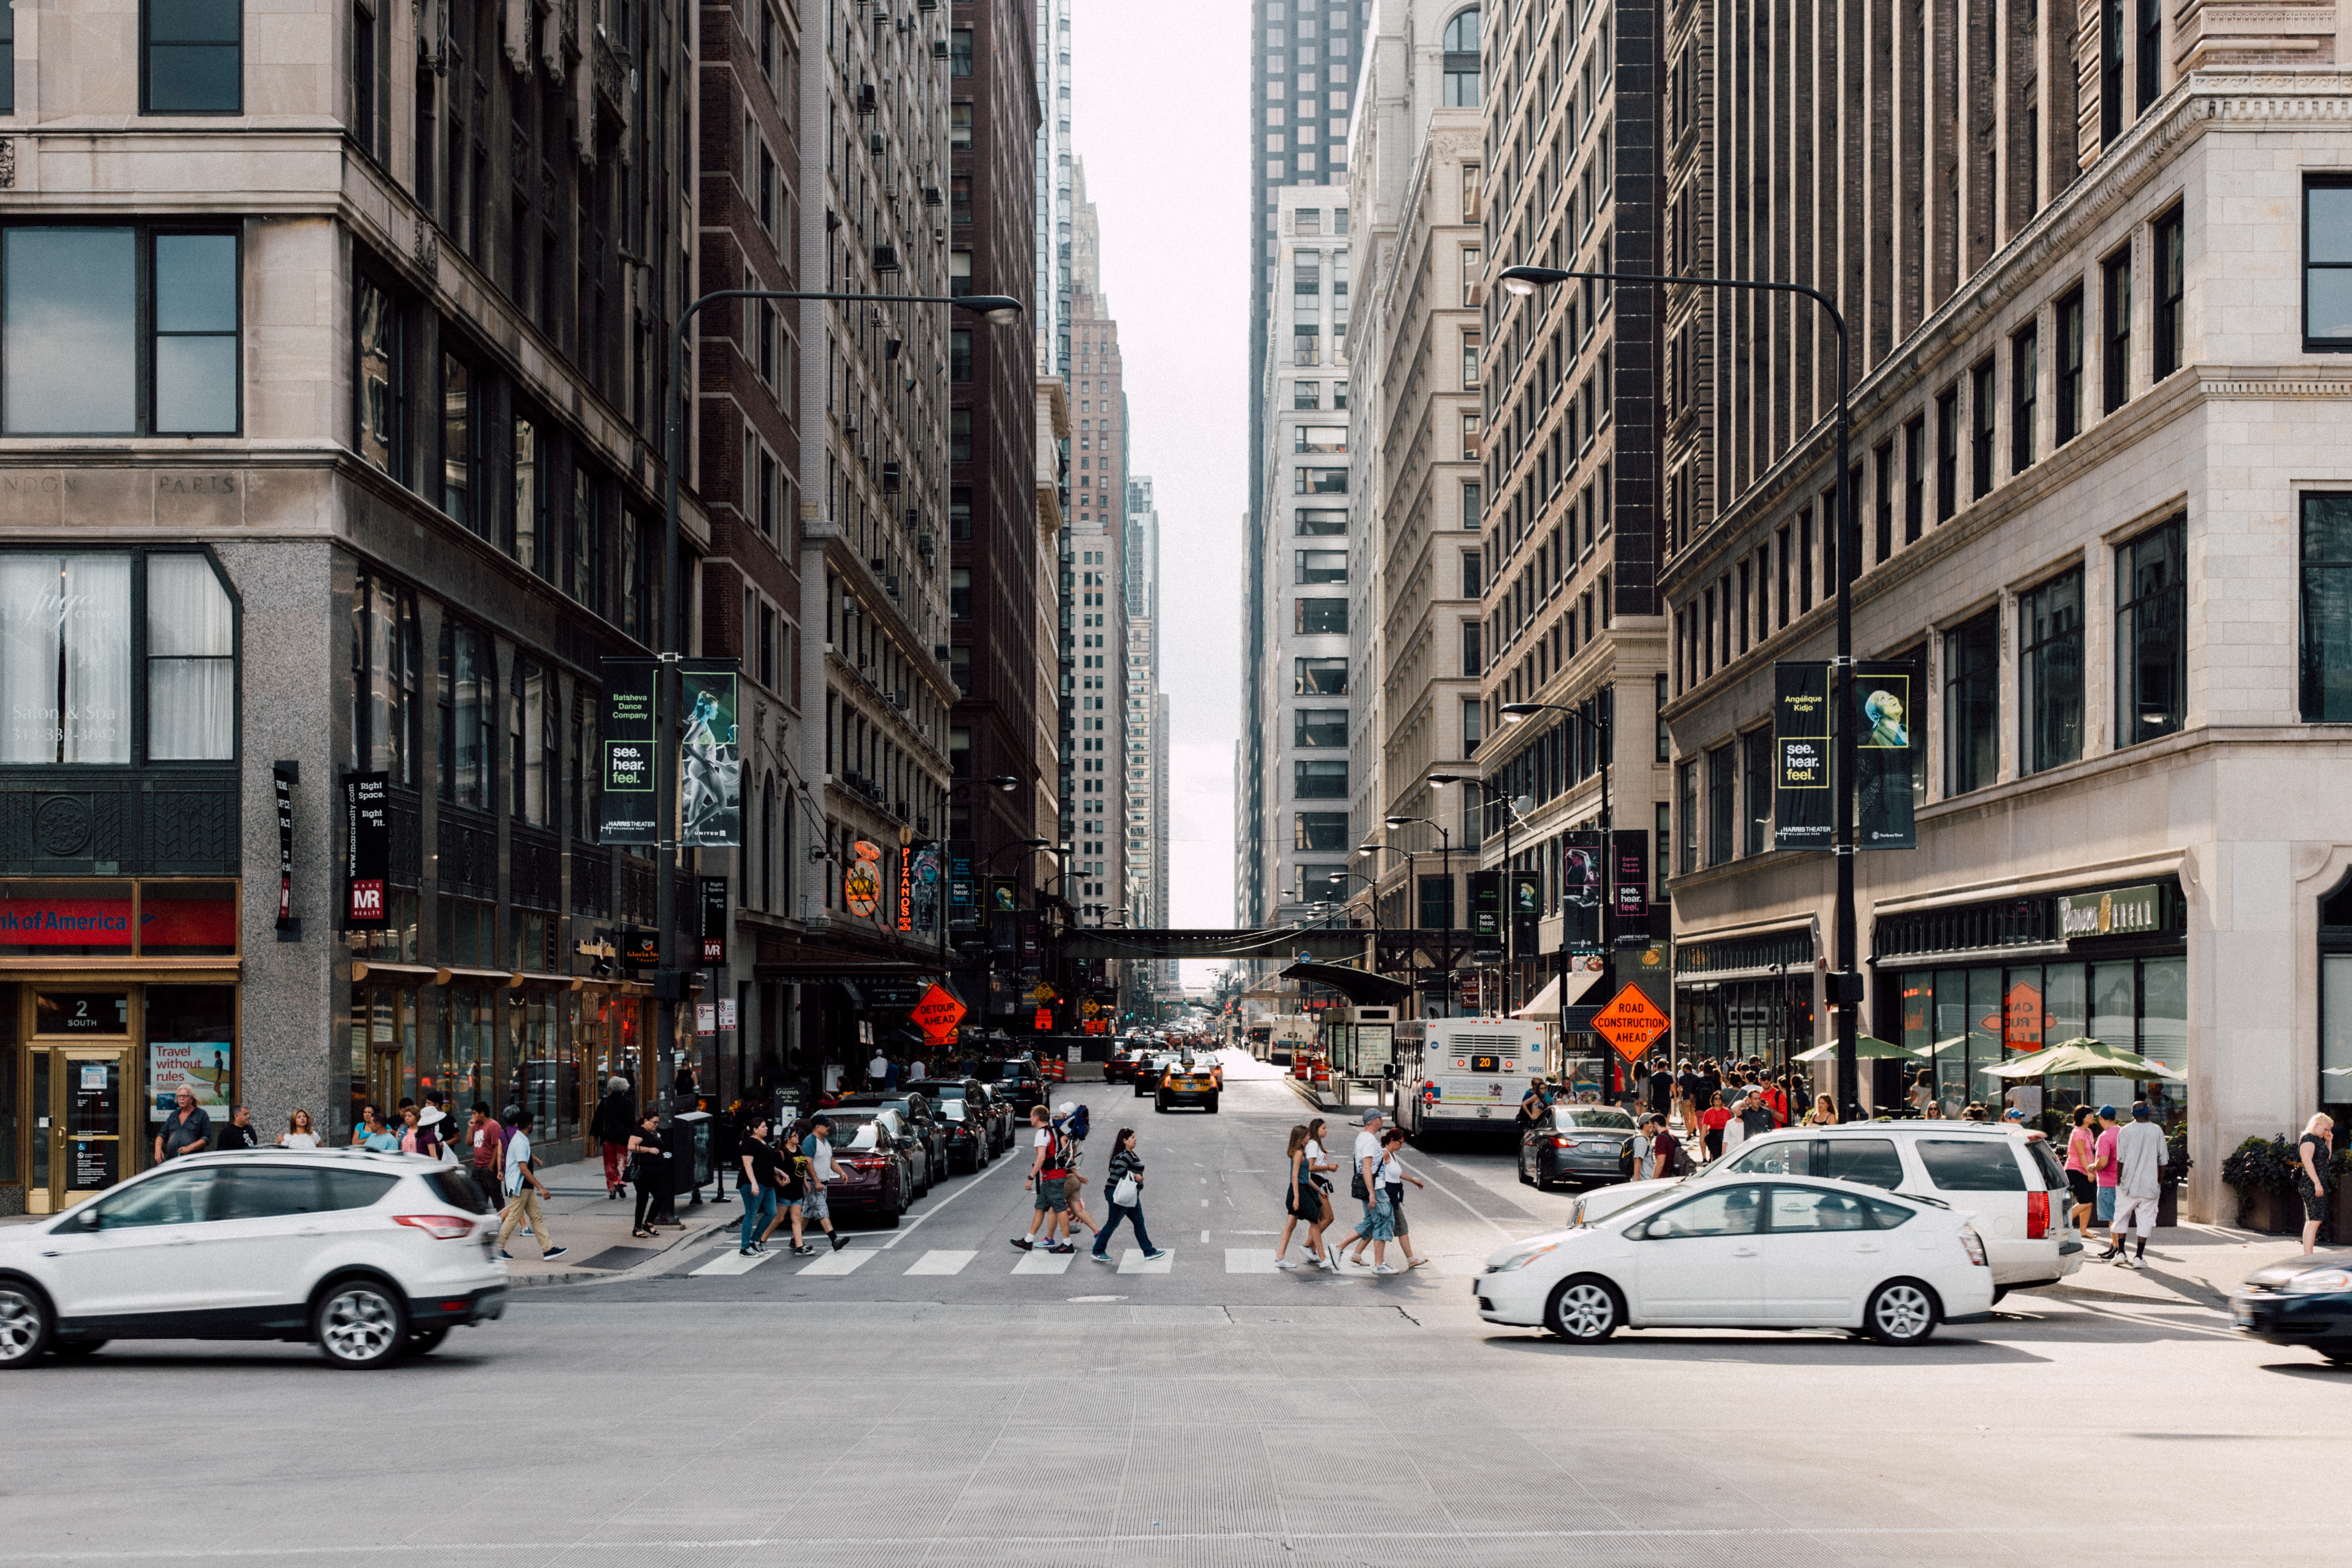
\includegraphics[height=0.3\textheight,keepaspectratio]{week3-input-yolo-1.jpg}
  \caption{Input}
\end{subfigure}
\begin{subfigure}{1\textwidth}
  \centering
  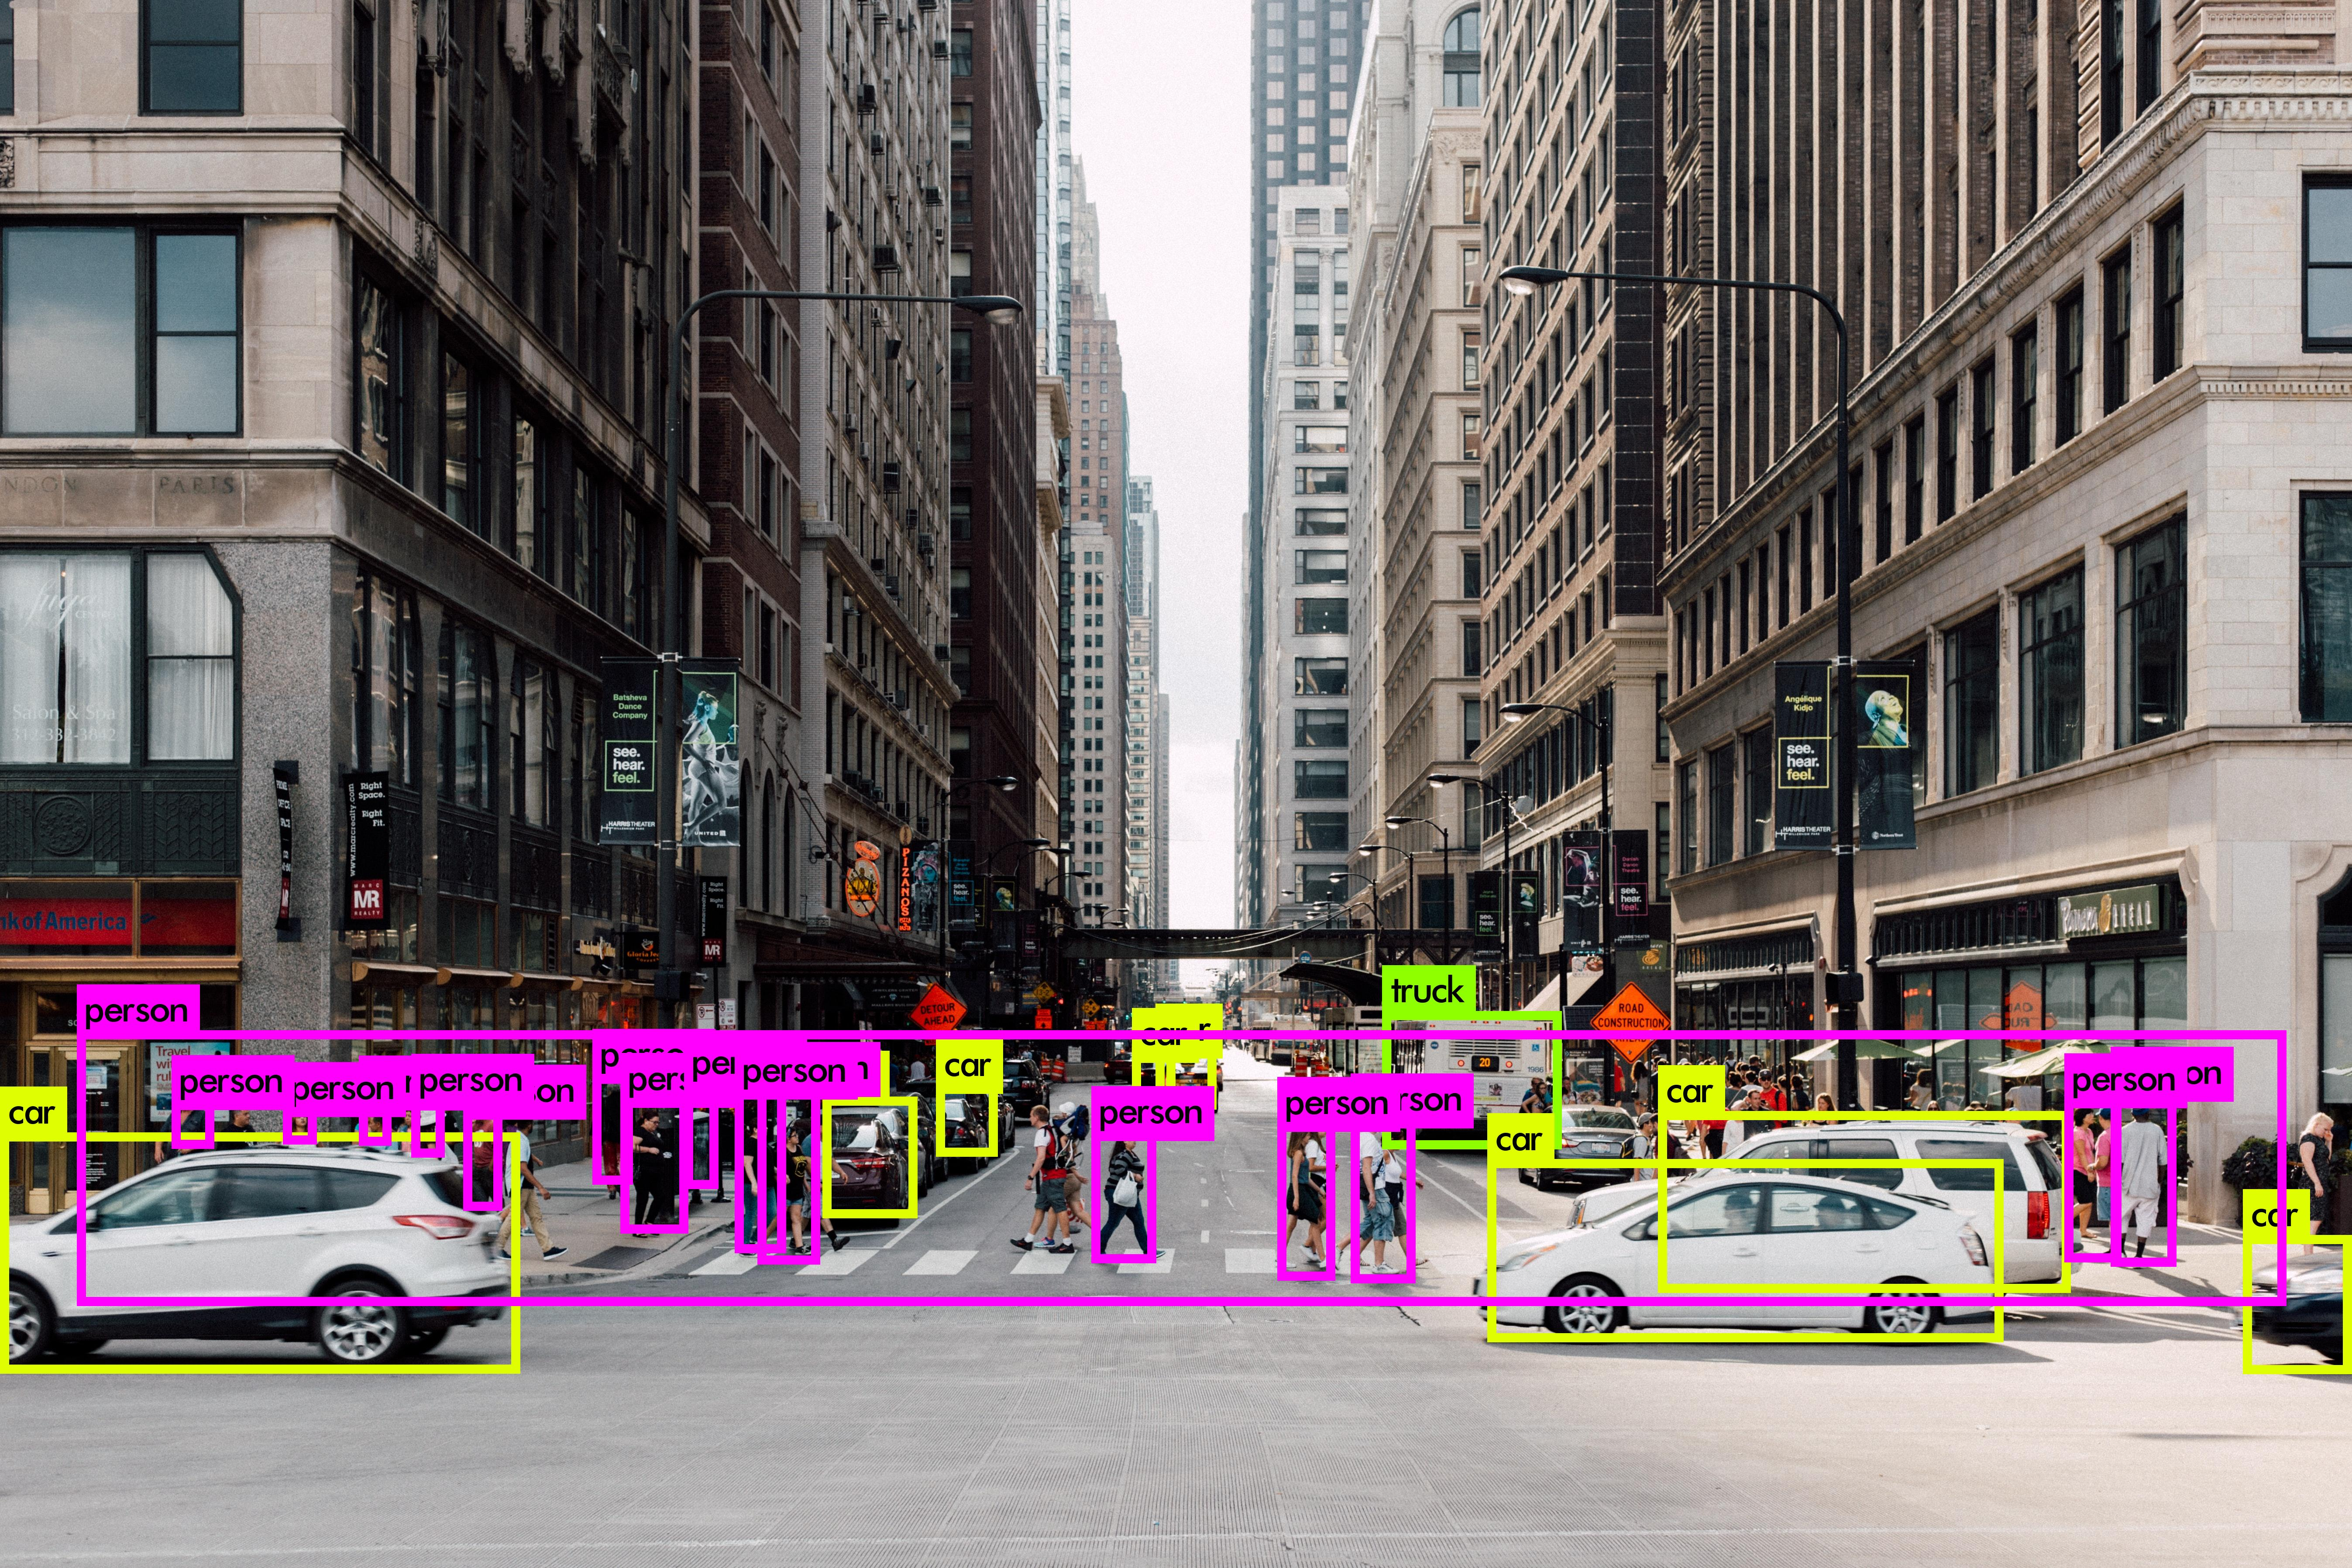
\includegraphics[height=0.3\textheight,keepaspectratio]{week3-yolo-1.jpg}
  \caption{Output}
\end{subfigure}
\caption{YOLO Object Detection}
\end{figure}

\subsection{Problems}
I built successfully OpenCV from source, but I was not able to build YOLO with OpenCV so I could not test YOLO with video or real-time camera.

How to make a Java wrapper for YOLO to run it on Android devices?